\section{pbrt:系统概述}\label{sec:pbrt:系统概述}

pbrt是使用标准的\keyindex{面向对象}{object-oriented}{}技术构建的:
重要实体都定义了抽象\keyindex{基类}{base class}{class类}(例如
抽象基类\refvar{Shape}{}定义了所有几何形状必须实现的接口,
光源的抽象基类\refvar{Light}{}也有相似设计)。
系统大部分都是纯粹由这些抽象基类提供的接口来实现的;
例如检查光源与着色点之间遮挡物体的代码
调用\refvar{Shape}{}的相交方法
而不要考虑场景中出现的特定类型的形状。
这种方式使得扩展系统变得很容易,
新增一种形状只需要实现一个完成\refvar{Shape}{}接口的类并链接到系统。

pbrt用10个关键抽象基类写成,列于\reftab{1.1}。
向系统添加这些类的新实现很简单;
实现必须从适当的基类继承,
编译和链接到可执行文件,
且必须修改附录第\refchap{场景描述接口}中的对象创建例程
以创建解析场景描述文件所需要的对象。
\refsec{添加新物体的实现}
\sidenote{译者注:原书此处似乎链接错误,已纠正。}
将讨论这种扩展系统的方法的更多细节。


\begin{table}[h]
    \centering
    \begin{tabular}{l l l}
        \toprule
        \textbf{基类}         & \textbf{目录}           & \textbf{章节}                   \\
        \midrule
        \refvar{Shape}{}      & \ttfamily shapes/       & \refsec{基本形状接口}           \\
        \refvar{Aggregate}{}  & \ttfamily accelerators/ & \refsec{聚合}                   \\
        \refvar{Camera}{}     & \ttfamily cameras/      & \refsec{相机模型}               \\
        \refvar{Sampler}{}    & \ttfamily samplers/     & \refsec{采样接口}               \\
        \refvar{Filter}{}     & \ttfamily filters/      & \refsec{图像重构}               \\
        \refvar{Material}{}   & \ttfamily materials/    & \refsec{材质接口与实现}         \\
        \refvar{Texture}{}    & \ttfamily textures/     & \refsec{纹理接口与基本纹理}     \\
        \refvar{Medium}{}     & \ttfamily media/        & \refsec{介质}                   \\
        \refvar{Light}{}      & \ttfamily lights/       & \refsec{光源接口}               \\
        \refvar{Integrator}{} & \ttfamily integrators/  & \refsub{积分器接口与采样积分器} \\
        \bottomrule
    \end{tabular}
    \caption{主要接口类型。pbrt大部分由此处列出的10个关键抽象基类实现。
        每个的实现都很容易添加到系统中扩展其功能。}
    \label{tab:1.1}
\end{table}

pbrt源码发布于\href{https://pbrt.org/}{\ttfamily pbrt.org}。
(大量场景示例\footnote{\url{http://pbrt.org/scenes-v3.html}}也可分开下载。)
所有的pbrt核心代码均在目录{\ttfamily src/core}内,
函数\refvar{main}{()}在
短文件\href{https://github.com/mmp/pbrt-v3/tree/master/src/main/pbrt.cpp}{\ttfamily main/pbrt.cpp}内。
抽象基类实例的各种实现在分开的目录下:
{\ttfamily src/shapes}有基类\refvar{Shape}{}的实现,
{\ttfamily src/materials}有基类\refvar{Material}{}的实现,以此类推。

本节有许多pbrt扩展版本渲染的图像。
其中从\reffig{1.11}到\reffig{1.14}
\sidenote{译者注:原书\reffig{1.14}引用文献似乎遗漏了链接,推测是\citep{10.1145/74334.74361}。}
都引人瞩目:
它们不仅令人过目不忘,而且每张都是渲染课程的学生在
最后的课程作业中对pbrt扩展新功能渲染得到的有趣图像。
这些是课程中最佳图像的一部分。
\begin{figure}[ht]
    \centering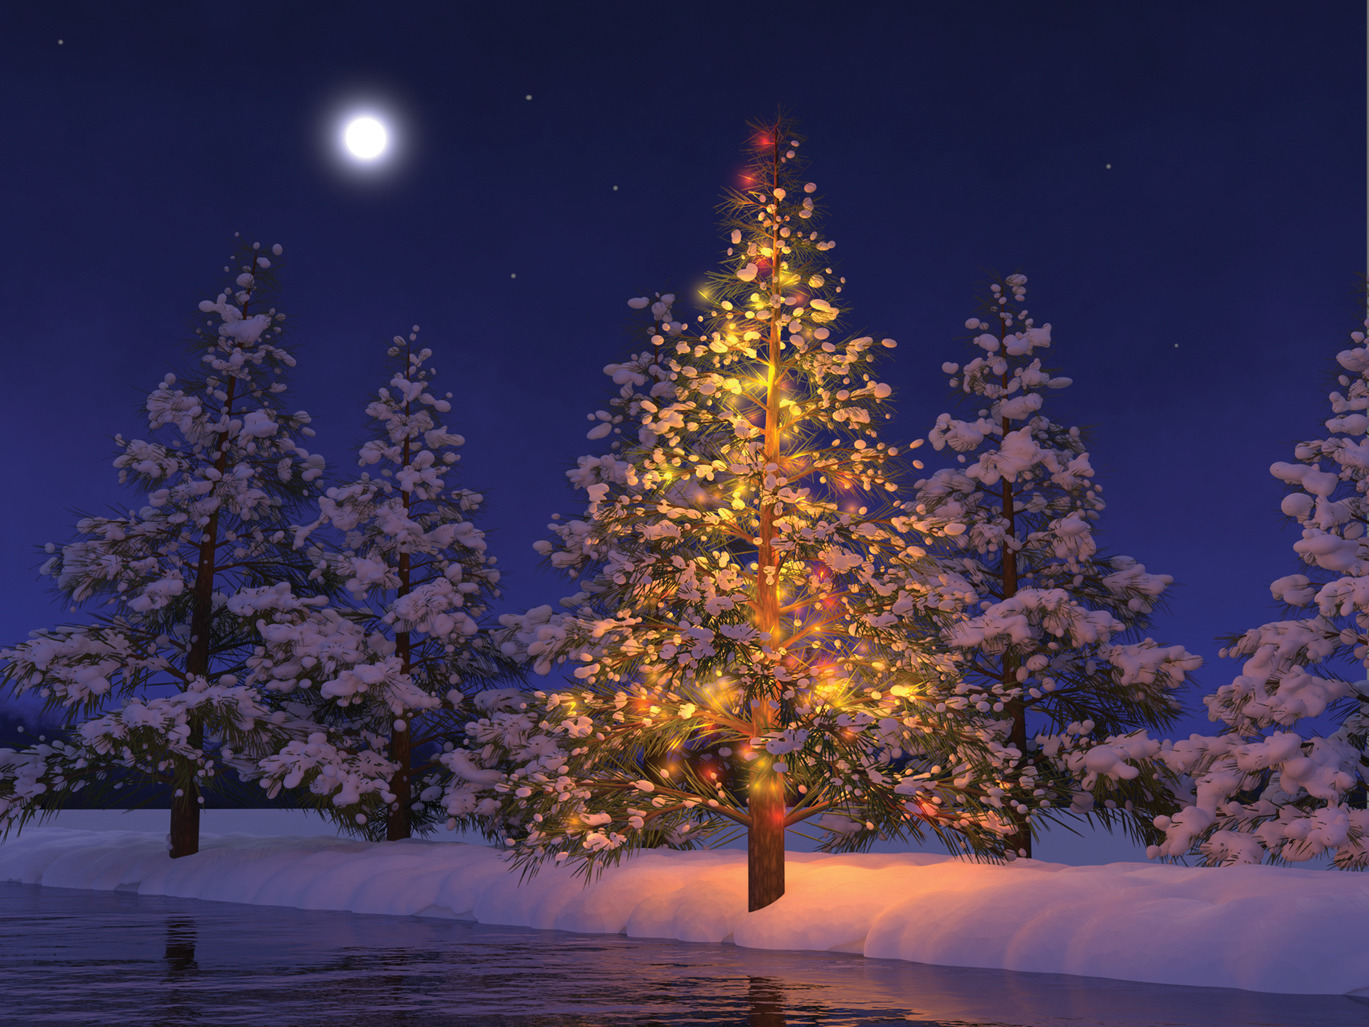
\includegraphics[width=\linewidth]{chap01/nightsnow.jpg}
    \caption{Guillaume Poncin和Pramod Sharma用许多方法扩展了pbrt,
        实现了一系列复杂渲染算法,
        制作出这张斯坦福大学CS348b渲染竞赛获奖图像。
        树木由L系统程序化建模,
        辉光图像处理滤波器增加了树上灯光的真实感,
        雪由metaball程序化建模,
        次表面散射算法考虑了光在离开雪前在雪下传播了一段距离的影响,
        赋予了雪逼真的外观。}
    \label{fig:1.11}
\end{figure}
\begin{figure}[ht]
    \centering
\includegraphics[width=\linewidth]{chap01/icecave.png}
    \caption{Abe Davis、David Jacobs和Jongmin Baek渲染了这张惊艳的冰窟图像,
        夺得2009斯坦福大学CS348b渲染竞赛大奖。
        他们首先实现了对冰川作用,即雪多年落下、融化、再冻结形成分层冰层这一物理过程的仿真。
        然后他们模拟了融水径流对冰的侵蚀,生成了冰的几何模型。
        体积内的光散射由体积光子映射模拟;
        冰的蓝色完全取决于在冰体中对依赖于波长的光吸收的建模。}
    \label{fig:1.12}
\end{figure}
\begin{figure}[ht]
    \centering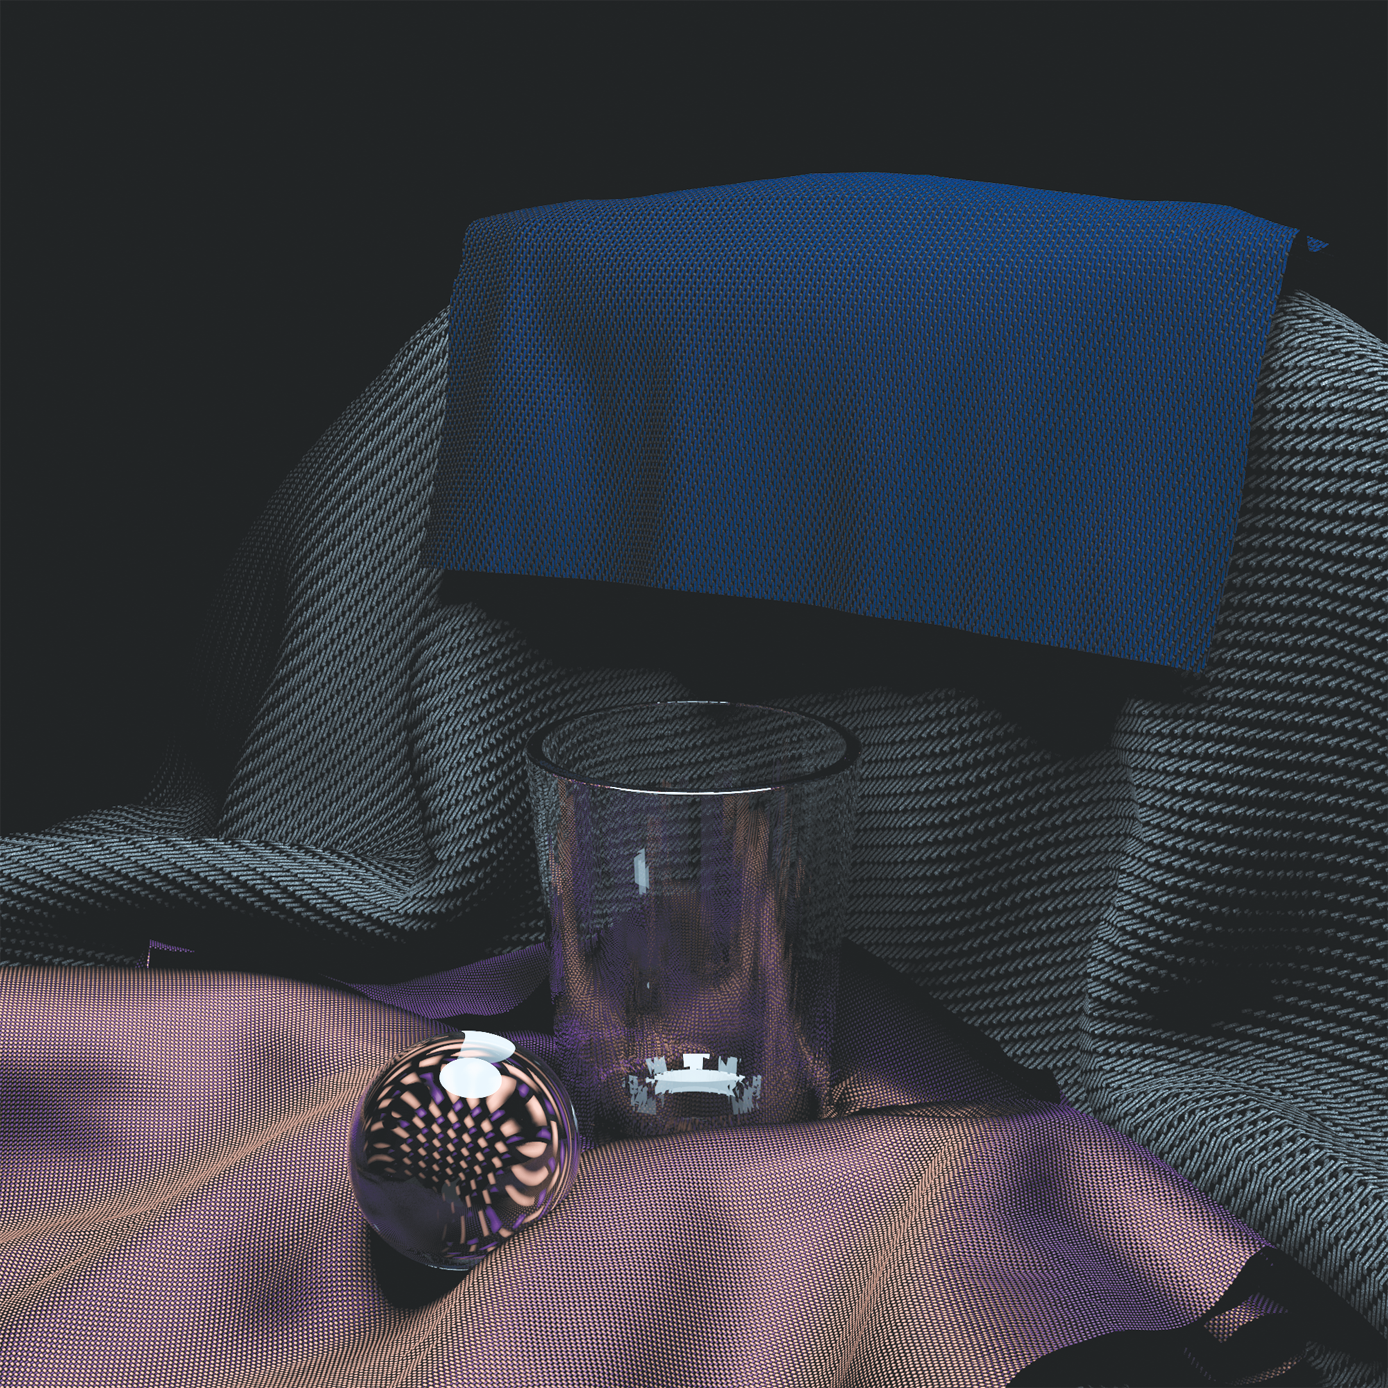
\includegraphics[width=\linewidth]{chap01/cloth.png}
    \caption{Lingfeng Yang实现了双向纹理函数来模拟布料的外观,
        添加了解析的自阴影模型,
        渲染了这张2009斯坦福大学CS348b渲染竞赛一等奖图像。}
    \label{fig:1.13}
\end{figure}

\subsection{执行阶段}\label{sub:执行阶段}

pbrt在概念上可分为两个执行阶段。
首先,解析用户提供的场景描述文件。
场景描述是一个文本文件,
指定了构成场景的几何形状及其材质属性、
对其照明的光源、虚拟相机在场景中的摆放位置、
整个系统所用的各个算法的参数等。
输入文件的每个语句都直接映射到
附录第\refchap{场景描述接口}
\sidenote{译者注:原书此处似乎链接错误,已纠正。}
中的一个例程;
这些例程包含了描述场景的程序接口。
场景文件格式的文档详见pbrt网站\href{https://pbrt.org/}{\ttfamily pbrt.org}。

解析阶段的最终结果是类\refvar{Scene}{}和\refvar{Integrator}{}的实例。
\refvar{Scene}{}包含了场景内容(几何物体、光源等)的表示,
\refvar{Integrator}{}则实现渲染它的算法。\keyindex{积分器}{integrator}{}这样命名的原因是
它的主要任务就是计算\refeq{1.1}的积分。

一旦指定好场景,第二执行阶段就开始了,执行主渲染循环。
pbrt通常把绝大部分运行时间都花在这个阶段,
本书大部分都在讲解执行这一阶段的代码。
渲染循环由{\ttfamily Integrator::}\refvar{Render}{()}的
实现来执行,它是\refsub{主渲染循环}的重点。

本章将介绍\refvar{Integrator}{}的一个特定子类,
称为\refvar{SamplerIntegrator}{},
其{\ttfamily Render()}方法为大量建模成像过程的光线
决定到达虚拟胶片平面的光量。
在计算完所有这些胶片样本的贡献后,最终图像被写入文件。
内存里的场景描述数据被释放,
系统从场景描述文件恢复处理语句直达没有剩余,
如果需要,用户可以指定下一个要渲染的场景。

\begin{figure}[ht]
    \centering\includegraphics[width=\linewidth]{chap01/furrydog.png}
    \caption{Jared Jacobs和Michael Turitzin为pbrt增加了
        Kajiya和Kay基于纹素的毛发渲染算法\citep{10.1145/74334.74361}并渲染了该图像,
        狗毛和粗毛地毯都是用纹素毛发算法渲染的。}
    \label{fig:1.14}
\end{figure}

\reffig{1.15}和\reffig{1.16}由\emph{LuxRender}渲染,
它是最初基于本书第一版pbrt源码的GPL许可的基于物理的渲染系统
(关于\emph{LuxRender}的更多信息详见\url{https://luxcorerender.org}
\sidenote{译者注:\emph{LuxRender}已更名为\emph{LuxCoreRender}且
    迁移到了新网址。此处已更正了网址,原书所给网址已经与\emph{LuxRender}无关了。})。

\begin{figure}[ht]
    \centering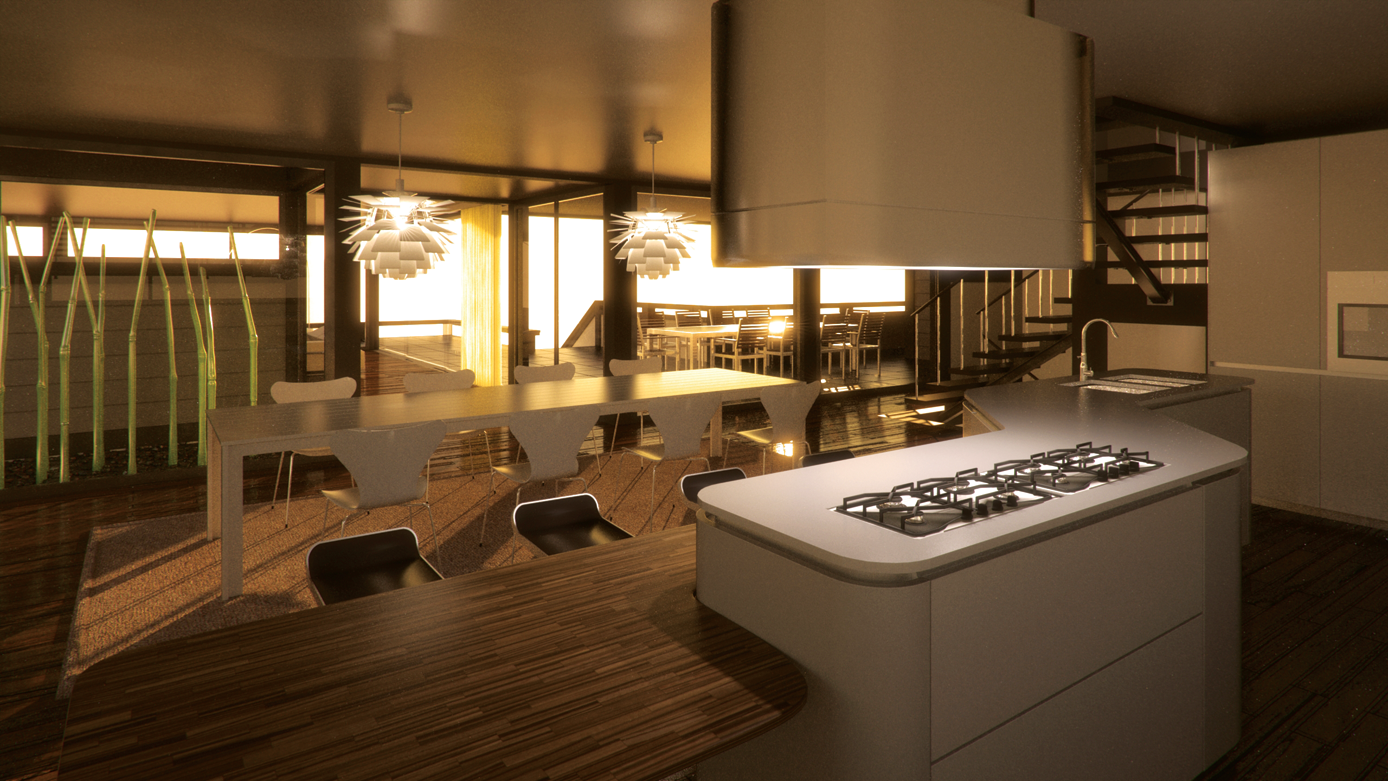
\includegraphics[width=\linewidth]{chap01/measure-one180-cut1260.png}
    \caption{Florent Boyer渲染了这个当代室内场景。
        该图像由\emph{LuxRender}渲染,它是最初
        基于pbrt源码的GPL许可的基于物理的渲染系统。
        建模和纹理由Blender完成。}
    \label{fig:1.15}
\end{figure}

\begin{figure}[ht]
    \centering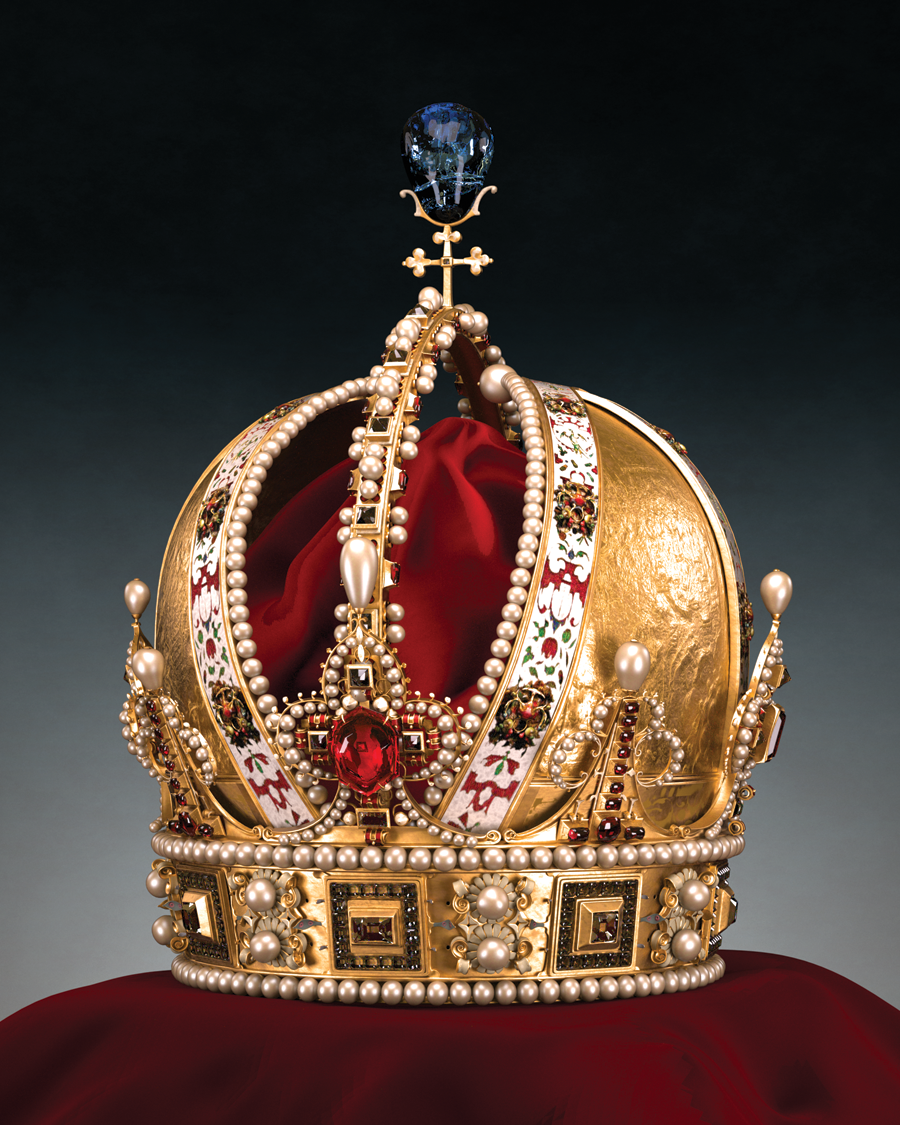
\includegraphics[width=\linewidth]{chap01/crown.png}
    \caption{Martin Lubich构建了这个奥地利皇冠的场景
        并用pbrt代码库的开源分支\emph{LuxRender}渲染了它。
        该场景由Blender建模,包含约一百八十万个顶点。
        它由具备基于真实世界光源测量数据的发射光谱的六个面光源照明,
        在四核CPU上对每个像素做1280次采样经73小时的计算完成渲染。
        包括可下载的Blender场景文件在内的更多信息
        详见Martin的网站\url{www.loramel.net}。}
    \label{fig:1.16}
\end{figure}

\subsection{场景表示}\label{sub:场景表示}
pbrt的函数\refvar{main}{()}可在
文件\href{https://github.com/mmp/pbrt-v3/tree/master/src/main/pbrt.cpp}{\ttfamily main/pbrt.cpp}内找到。
该函数很简单;
它首先循环读取{\ttfamily argv}中的命令行参数,
初始化结构体{\ttfamily Options}中的值并
保存参数中的文件名。
运行pbrt时带命令行参数{\ttfamily -help}会
打印所有可指定的命令行选项。
解析命令行参数的代码片\refcode{Process command-line arguments}{}很简单,
故本书不再介绍\sidenote{译者注:我还是把它搬上来了。}。

选项结构体随后传入函数\refvar{pbrtInit}{()},做全系统初始化。
函数\refvar{main}{()}再解析给定场景描述,
创建\refvar{Scene}{}和\refvar{Integrator}{}。
\refvar{pbrtCleanup}{()}在系统完成所有渲染后退出前做最后的清理工作。

函数\refvar{pbrtInit}{()}和\refvar{pbrtCleanup}{()}出现在
页边空白处的迷你索引内,还注明了真正定义它们的页数。
每页的迷你索引都指向了所用的几乎所有函数、类、方法和成员变量的定义
\sidenote{译者注:我不太理解所谓的迷你索引是什么,
    不过翻译时竭力还原了在线版的跳转功能。
    例如这里的\refvar{main}{()}的函数体内
    有不少地方是可以单击跳转的。
    此外正文部分也有这种功能。试试看吧!}。
\begin{lstlisting}
`\initcode{Main program}{=}`
int `\initvar{main}{}`(int argc, char *argv[]) {
    Options options;
    std::vector<std::string> filenames;
    `\refcode{Process command-line arguments}{}`
    `\refvar{pbrtInit}{}`(options);
    `\refcode{Process scene description}{}`
    `\refvar{pbrtCleanup}{}`();
    return 0;
}
\end{lstlisting}

\begin{lstlisting}
`\initcode{Process command-line arguments}{=}`
for (int i = 1; i < argc; ++i) {
    if (!strcmp(argv[i], "--ncores") || !strcmp(argv[i], "--nthreads"))
        options.nThreads = atoi(argv[++i]);
    else if (!strcmp(argv[i], "--outfile")) options.imageFile = argv[++i];
    else if (!strcmp(argv[i], "--quick")) options.quickRender = true;
    else if (!strcmp(argv[i], "--quiet")) options.quiet = true;
    else if (!strcmp(argv[i], "--verbose")) options.verbose = true;
    else if (!strcmp(argv[i], "--help") || !strcmp(argv[i], "-h")) {
        printf("usage: pbrt [--nthreads n] [--outfile filename] [--quick] [--quiet] "
               "[--verbose] [--help] <filename.pbrt> ...\n");
        return 0;
    }
    else filenames.push_back(argv[i]);
}
\end{lstlisting}

如果运行pbrt时没有提供输入文件名,
则它会从标准输入读取场景描述。
否则它就遍历提供的文件名,依次处理每个文件。
\begin{lstlisting}
`\initcode{Process scene description}{=}`
if (filenames.size() == 0) {
    `\refcode{Parse scene from standard input}{}`
} else {
    `\refcode{Parse scene from input files}{}`
}
\end{lstlisting}
函数{\initvar{ParseFile}{()}}或从标准输入或磁盘文件读入并解析场景描述文件;
如果无法打开文件则返回{\ttfamily false}。
本书不介绍解析场景描述文件的机制;
解析器的实现可在文件\href{https://github.com/mmp/pbrt-v3/blob/master/src/core/parser.h}{\ttfamily core/parser.h}和
\href{https://github.com/mmp/pbrt-v3/blob/master/src/core/parser.cpp}{\ttfamily core/parser.cpp}中找到
\sidenote{译者注:此处已更正文件名,因为原书给出的文件名已经失效了。}。
想要了解解析子系统但不熟悉这些工具的读者可以参阅Levine、Mason和Brown的著作\citep{10.5555/136311}。

我们遵循的UNIX习惯用法,以名为“{\ttfamily -}”的文件表示标准输入:
\begin{lstlisting}
`\initcode{Parse scene from standard input}{=}`
`\refvar{ParseFile}{}`("-");
\end{lstlisting}

如果无法打开特定的输入文件,则\refvar{Error}{()}例程会将此信息报告给用户。
\refvar{Error}{()}使用和{\ttfamily printf()}相同的格式化字符串语义。
\begin{lstlisting}
`\initcode{Parse scene from input files}{=}`
for (const std::string &f : filenames)
    if (!`\refvar{ParseFile}{}`(f))
        `\refvar{Error}{}`("Couldn't open scene file \"%s\"", f.c_str());
\end{lstlisting}

解析完场景文件后就创建表示场景中光源和几何图元的对象。
它们都存与\refvar{Scene}{}对象中,
由附录\refsub{世界端和渲染}的方法\refvar{RenderOptions::MakeScene}{()}创建。
类\refvar{Scene}{}在\href{https://github.com/mmp/pbrt-v3/tree/master/src/core/scene.h}{\ttfamily core/scene.h}中
声明并在\href{https://github.com/mmp/pbrt-v3/tree/master/src/core/scene.cpp}{\ttfamily core/scene.cpp}中定义。
\begin{lstlisting}
`\initcode{Scene Declarations}{=}`
class `\initvar{Scene}{}` {
public:
    `\refcode{Scene Public Methods}{}`
    `\refcode{Scene Public Data}{}`
private:
    `\refcode{Scene Private Data}{}`
};
\end{lstlisting}

\begin{lstlisting}
`\initcode{Scene Public Methods}{=}\initnext{ScenePublicMethods}`
`\refvar{Scene}{}`(std::shared_ptr<`\refvar{Primitive}{}`> `\refvar{aggregate}{}`,
      const std::vector<std::shared_ptr<`\refvar{Light}{}`>> &`\refvar{lights}{}`)
    : `\refvar{lights}{}`(`\refvar{lights}{}`), `\refvar{aggregate}{}`(`\refvar{aggregate}{}`) {
    `\refcode{Scene Constructor Implementation}{}`
}
\end{lstlisting}

场景中每个光源都由\refvar{Light}{}对象表示,
指定灯光的形状和发射能量的分布。
\refvar{Scene}{}用C++标准库中{\ttfamily shared\_ptr}实例
的一个{\ttfamily vector}来存储所有光源。
pbrt用共享指针\sidenote{译者注:原文shared pointers,是一种智能指针。}跟踪
其他实例对对象的引用计数。
当最后一个持有引用的实例(例如这里的\refvar{Scene}{})被销毁时,
引用计数减到零,\refvar{Light}{}就可以安全释放了,而且是自动的。

尽管一些渲染器支持每个几何对象有单独的光源列表,
允许一个光源只照明场景中一部分物体,
但这种做法不符合pbrt采用的基于物理的渲染方法,
所以对于每个场景pbrt只支持单个全局列表。
系统的许多部分都需要获取光源,
所以\refvar{Scene}{}把它们置为公有成员变量。
\begin{lstlisting}
`\initcode{Scene Public Data}{=}`
std::vector<std::shared_ptr<`\refvar{Light}{}`>> `\initvar{lights}{}`;
\end{lstlisting}

场景中每个几何对象都由\refvar{Primitive}{}表示,结合了两个对象:
指定其几何结构的\refvar{Shape}{}和描述其外观
例如物体的颜色、是否具有暗淡或光泽饰面)的\refvar{Material}{}。
所有几何图元都集中到\refvar{Scene}{}的
成员变量\refvar{Scene}{::}\refvar{aggregate}{}这一
单个\refvar{Primitive}{}聚合体中。
这个聚合体是一种特殊的图元,它自己持有许多对其他图元的引用。
因为它实现了\refvar{Primitive}{}接口,
所以从单个图元到系统其余部分似乎没什么区别。
聚合体的实现以加速的数据结构存储了所有场景图元,
减少对远离给定光线的图元做不必要的光线交点测试的数量。
\begin{lstlisting}
`\initcode{Scene Private Data}{=}\initnext{ScenePrivateData}`
std::shared_ptr<`\refvar{Primitive}{}`> `\initvar{aggregate}{}`;
\end{lstlisting}
构造函数把场景几何的边框缓存到成员变量{\ttfamily worldBound}中。
\begin{lstlisting}
`\initcode{Scene Constructor Implementation}{=}\initnext{SceneConstructorImplementation}`
`\refvar{worldBound}{}` = aggregate->`\refvar{WorldBound}{}`();
\end{lstlisting}
\begin{lstlisting}
`\refcode{Scene Private Data}{+=}\lastcode{ScenePrivateData}`
`\refvar{Bounds3f}{}` `\initvar{worldBound}{}`;
\end{lstlisting}
可通过方法{\ttfamily WorldBound()}获取该边界。
\begin{lstlisting}
`\refcode{Scene Public Methods}{+=}\lastcode{ScenePublicMethods}`
const `\refvar{Bounds3f}{}` &WorldBound() const { return `\refvar{worldBound}{}`; }
\end{lstlisting}

一些光源实现发现在定义场景后开始渲染前做一些额外的初始化很有用。
{\ttfamily Scene}的构造函数调用其方法{\ttfamily Preprocess()}来允许它们这么做。
\begin{lstlisting}
`\refcode{Scene Constructor Implementation}{+=}\lastcode{SceneConstructorImplementation}`
for (const auto &light : `\refvar{lights}{}`)
    light->`\refvar{Preprocess}{}`(*this);
\end{lstlisting}

\refvar{Scene}{}类提供两个与光线-图元交点相关的方法。
它的{\ttfamily Intersect()}方法跟随给定光线到场景中并
返回表示光线是否与某一图元相交的布尔值。
如果是,它便把沿光线最近交点的信息填入提供的结构体\refvar{SurfaceInteraction}{}。
结构体\refvar{SurfaceInteraction}{}将在\refsec{图元接口与几何图元}定义。
\begin{lstlisting}
`\initcode{Scene Method Definitions}{=}\initnext{SceneMethodDefinitions}\htarget{codevar:Scene::Intersect}{}`
bool `\refvar{Scene}{}`::`\refvar{Intersect}{}`(const `\refvar{Ray}{}` &ray, `\refvar{SurfaceInteraction}{}` *isect) const {
    return `\refvar{aggregate}{}`->`\refvar{Intersect}{}`(ray, isect);
}
\end{lstlisting}
一个紧密相关的方法是\refvar{Scene::IntersectP}{()},
它沿光线检查交点的存在性但不返回任何关于这些交点的信息。
因为这个例程不需要搜索最近的交点或计算任何关于交点的额外信息,
所以它一般比\refvar{Scene::Intersect}{()}更高效。
这个例程用于阴影射线。
\begin{lstlisting}
`\refcode{Scene Method Definitions}{+=}\lastnext{SceneMethodDefinitions}\htarget{codevar:Scene::IntersectP}{}`
bool `\refvar{Scene}{}`::`\refvar{IntersectP}{}`(const `\refvar{Ray}{}` &ray) const {
    return `\refvar{aggregate}{}`->`\refvar{IntersectP}{}`(ray);
}
\end{lstlisting}

\subsection{积分器接口与采样积分器}\label{sub:积分器接口与采样积分器}

\begin{lstlisting}
`\initcode{Integrator Declarations}{=}`
class `\initvar{Integrator}{}` {
public:
    `\refcode{Integrator Interface}{}`
};
\end{lstlisting}

\begin{lstlisting}
    `\initcode{Integrator Interface}{=}`
    virtual void `\initvar{Render}{(const \refvar{Scene}{} \&scene)}` = 0;
\end{lstlisting}

\begin{lstlisting}
`\initcode{SamplerIntegrator Declarations}{=}`
class `\initvar{SamplerIntegrator}{}` : public `\refvar{Integrator}{}` {
public:
    `\refcode{SamplerIntegrator Public Methods}{}`
protected:
    `\refcode{SamplerIntegrator Protected Data}{}`
private:
    `\refcode{SamplerIntegrator Private Data}{}`
};
\end{lstlisting}


\subsection{主渲染循环}\label{sub:主渲染循环}
